\documentclass{article}

% Packages
\usepackage{titling}
\usepackage[utf8]{inputenc}
\usepackage[english]{babel}
\usepackage{amsmath,amssymb}
\usepackage{graphicx}
\usepackage{float}
\usepackage{subcaption}
\usepackage[hidelinks]{hyperref}
\usepackage{xcolor}
\usepackage{listings}
\usepackage[a4paper, top = 2cm, bottom = 2cm, left = 2cm, right = 2cm]{geometry}
\usepackage{multicol}
\usepackage{booktabs}
\usepackage{array}



\graphicspath{{Figures/}}
\newcolumntype{M}[1]{>{\centering\arraybackslash}m{#1}}



% Title page information
\pretitle{
  \begin{center}
  \LARGE
  
\includegraphics[width=15.1cm,height=3.05cm]{Logo_unipv.png}\vspace*{1cm}\\[\bigskipamount]}


\title{\Large Machine Learning Course\vspace{0.8cm}\\
    \rule{\textwidth}{0.3pt}\vspace{0.3cm}\\
    \textbf{Speech Commands Recognition}\vspace{0.1cm}\\
    \rule{\textwidth}{0.3pt}\vspace{0.8cm}}

\posttitle{\end{center}}
    
\author{Andrea Alberti\vspace{0.5cm}\\
    \small Department of Computer Engineering - Data Science\\[0.2cm]
    \small University of Pavia, Italy \\
    \small Email: andrea.alberti01@universitadipavia.it}\vspace{0.5cm}
        
\date{\today}

\begin{document}

\begin{titlepage}
   
        \maketitle
        \thispagestyle{empty}

    \begin{multicols*}{2}
            
        \hrule
        \begin{abstract}
        \noindent
        This project aimed to develop a highly accurate speech recognition model capable of distinguishing between 35 different spoken words, trained on a 
        dataset comprising 105,829 audio recordings by numerous speakers. \\
        To achieve this objective, various MLP architectures were evaluated, resulting in 
        a test accuracy of approximately 49\%. However, the task's complexity, with numerous classes to classify, posed a significant challenge in developing 
        a robust model. Additionally, some words had fewer recordings, which adversely impacted the overall model performance. 
        The model choice was based on the comparison between different model's architectures and normalization techniques.
        The project provides insights about the significance of addressing dataset imbalances, the importance of feature normalization, and the 
        performance of an MLP model on the speech recognition task.
        \\
        \\
        \\
        \end{abstract}
     \newcolumn
        \hrule\vspace{0.1cm}
        \tableofcontents
    \end{multicols*}

\end{titlepage}

\newpage
\pagenumbering{arabic}



%---------------------------------------------------------

\begin{multicols}{2}
    
\section{Introduction}
This project is about the implementation of a Neural Network for the classification of audio files. This problem is known as \textit{Speech Command Recognition} and its importance has been raising 
in the last years thanks to the development of smart devices and the need of a more natural interaction with them. The main library exploited for the implementation is \textit{pvml}.

\subsection{Available Data}
The data set includes 105829 recordings of 35 words uttered by many different speakers. For the analysis it is divided into three subsets: \textit{train}, \textit{validation} and \textit{test}.

\subsection{Goal}
The goal is to fit on the data a Multi Layer Perceptron (MLP) so that it can be exploited to classify new unseen data on the 35 different classes.

\subsection{Multi Layer Perceptron}
A Multi Layer Perceptron (MLP) is a type of Feed Forward Neural Network that consists of zero or more hidden layers of interconnected neurons between an input layer and an output layer. 
Each neuron in an MLP receives input signals from all neurons in the previous layer, applies an activation function to the weighted sum of its inputs, and outputs the result to the next layer. 
The parameters of the MLP (weights and biases) are learned optimizing a chosen Loss Function (Cross Entropy) through a process called Backpropagation. 


%-----------------------------------------------------------

\section{Model Building}
Prior to start building the model is important to pre-process the data, making them suitable to be passed to the training algorithm. This process is known as \textit{Feature Extraction} and it is
a fundamental one in the model creation.

\subsection{Features Extraction}
Starting from the raw audio data, extraction of features consists in the creation of a spectrogram for each word. This latter has been made uniform in size by padding or truncating the original signals.

\subsection{Data Visualization}
To better understand the data, it is useful to visualize some of the spectrograms. In figure \ref{fig:spec_examples} are reported some examples about some words.
The red zones are those in which the frequencies are more present. It is important to underline that the same word can have different spectrograms depending on the speaker.

    \begin{figure}[H]
        \centering
        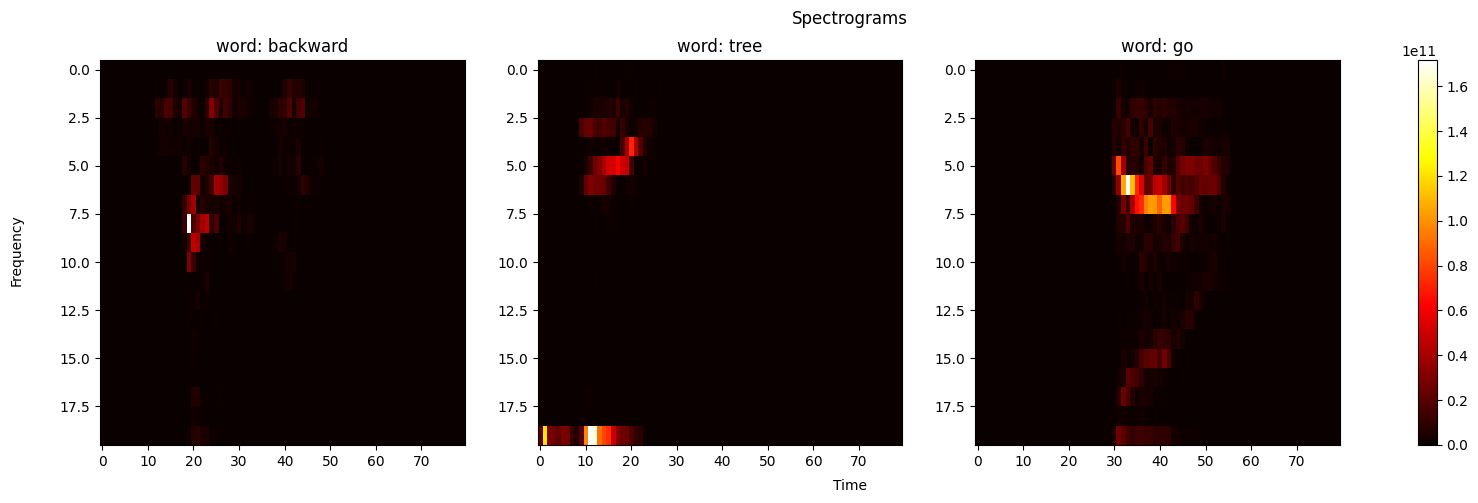
\includegraphics[width=0.48\textwidth]{spectrograms_sample.png}
        \caption{\small Spectrograms example }
        \label{fig:spec_examples}
    \end{figure}

\subsection{Feature Normalization}
Another important step in the pre-processing phase is the normalization of the features. Among the several normalization techniques available, the four used in this project 
are \textit{Mean-Var}, \textit{Min-Max}, \textit{Whitening} and \textit{Max-Abs} normalization. All these methods are compared in figure \ref{fig:normcomptest}. 
It is evident that the best one is the Mean-Variance normalization.
This is because it helps to reduce the impact of differences in the volume or intensity of the audio recordings, centering the data around zero and 
scaling them to have unit variance. These normalized data allow the model to capture underlying patterns.

    \begin{figure}[H]
        \centering
        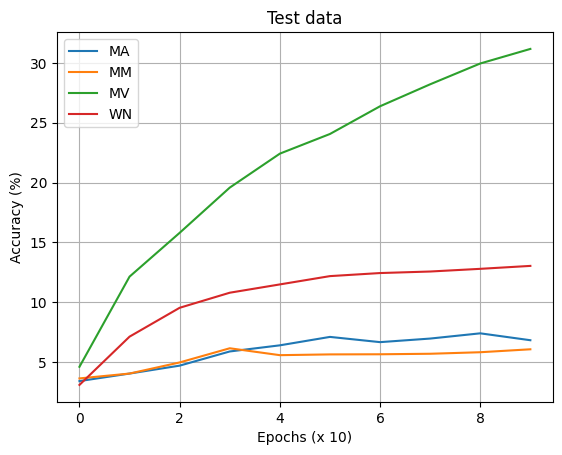
\includegraphics[width=0.48\textwidth]{norm_comp_test.png}
        \caption{\small Normalization comparison}
        \label{fig:normcomptest}
    \end{figure}


\subsection{Train Classifier}

\textbf{Batch size}\\
To optimize the training the data are divided into mini-batches. The size of the batch could impact on the model performance, therefore different
values have been tested and the result are reported in figure \ref{fig:bcte}. The used model had not hidden layers, therefore its performance is poor, thus
all the sizes converges to 18\% accuracy on the test set but requiring different number of epochs. The fastest was the 50 batch size and it is chosen as the best one.

    \begin{figure}[H]
        \centering
        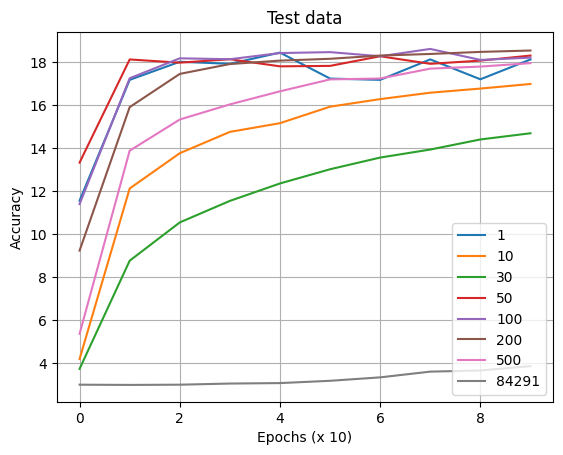
\includegraphics[width=0.48\textwidth]{batch_comp_test.png}
        \caption{\small Batch comparison}
        \label{fig:bcte}
    \end{figure}

\noindent
\textbf{Architecture}\\
The architecture of the network strongly influences its performance therefore different configurations results are compared in figure \ref{fig:acte}.
For time reasons, the number of epochs is limited to 100 disregarding that some networks have more parameters and could take more time to express
their full potential.
In this greedy approach the best architecture is that with many hidden layers. This type of architecture was trained with 400 epochs, in figure 
\ref{fig:chosencomp} are shown the results. The blue and orange model reached 80\% in training
accuracy, however, when tested on the independent test set, their performance was not as good, suggesting that they were overfitting to the training data.
To address this problem, several regularization values were tested, and a regularization parameter of $\lambda = 0.001$ was found to be the most effective. 
Despite this effort, overfitting was only slightly reduced, but not entirely resolved. Ultimately, the red model was selected as the best-performing model 
and used for further analysis.

    \begin{figure}[H]
        \centering
        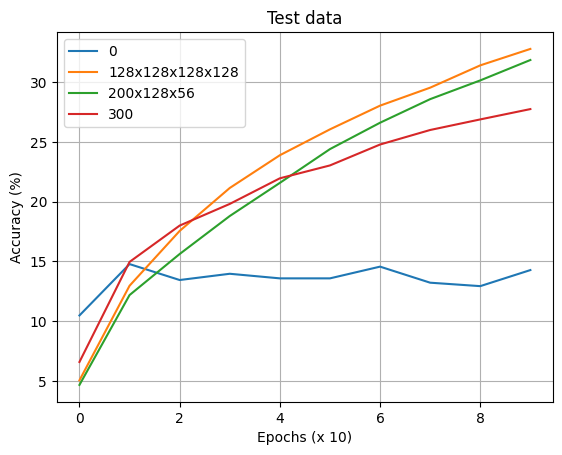
\includegraphics[width=0.48\textwidth]{arch_comp_test.png}
        \caption{\small Architecture comparison}
        \label{fig:acte}
    \end{figure}

    \begin{figure}[H]
        \centering
        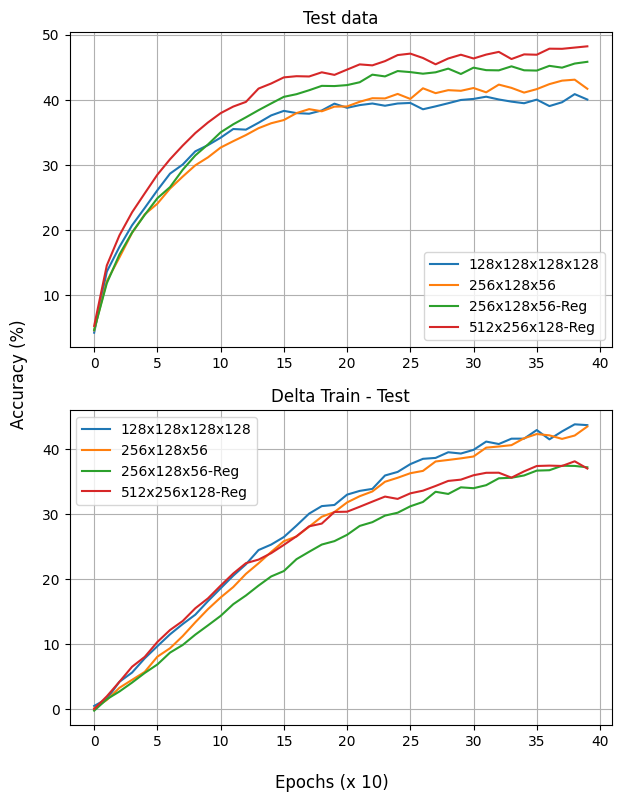
\includegraphics[width=0.48\textwidth]{chosen_comp_test_delta.png}
        \caption{\small Deep Networks comparison}
        \label{fig:chosencomp}
    \end{figure}


%-----------------------------------------------------------

\section{Model Analysis}
To analyze the behavior of the chosen model was created a confusion matrix in figure \ref{fig:confmat} that shows the number of correct and 
incorrect predictions for each class. The darker the color, the higher the number of samples of class i (row index) classified as class j (column index). As expected, the diagonal
is the most populated part of the matrix, meaning that the model correctly classifies a word lots of times. 

    \begin{figure}[H]
        \centering
        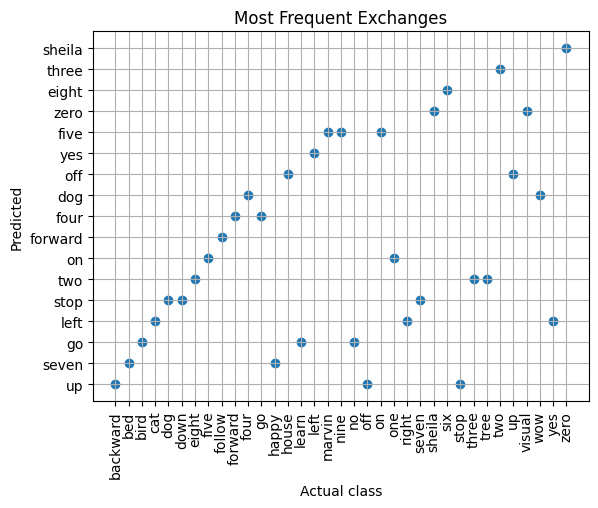
\includegraphics[width=0.48\textwidth]{mostex.png}
        \caption{\small Most exchanged}
        \label{fig:mostex}
    \end{figure}

\addcontentsline{toc}{subsection}{{Most Exchanged Classes}}
\noindent
\textbf{Most Exchanged Classes}\\
The most exchanged classes are those in which the model has more difficulties to distinguish between. In figure \ref{fig:mostex} are reported for each word the class to which
the model classifies them (excluded correct classifications) most of times. Lots of exchanges are reasonable like \textit{Forward} classified to \textit{Four} and
\textit{Three} to \textit{Two} whose spectrograms are very similar (figure \ref{fig:mostmis_ex}).

    \begin{figure}[H]
        \centering
        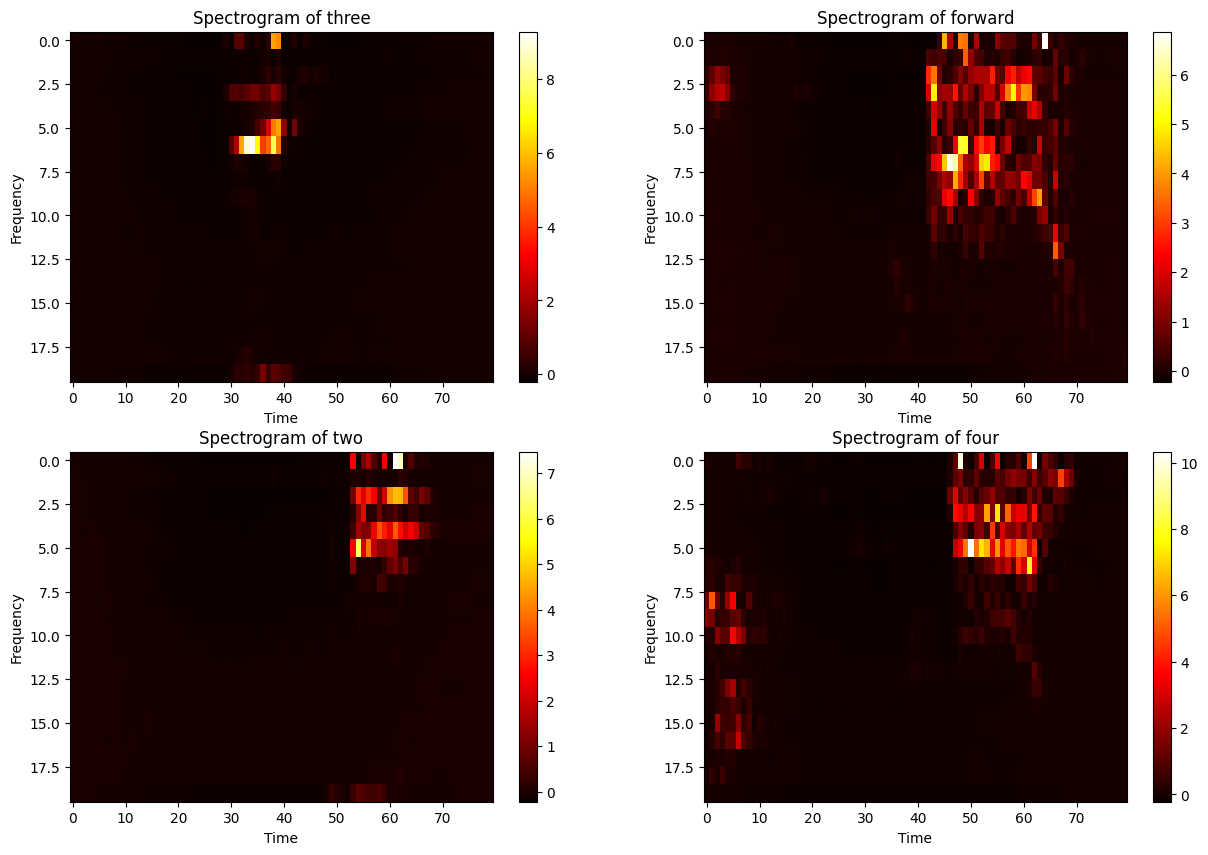
\includegraphics[width=0.48\textwidth]{mostmis_spec.png}
        \caption{\small Three VS Two, Forward VS Four}
        \label{fig:mostmis_ex}
    \end{figure}

\addcontentsline{toc}{subsection}{{Most Misclassified Samples}}
\noindent
\textbf{Most Misclassified Samples}\\
Some words are more difficult to be classified than others and in figure \ref{fig:mostmis} are reported the most misclassified samples. \textit{Tree} and \textit{Learn} are the most misclassified words, listening to 
the audio files of \textit{learn} it is possible to notice that lots of time the word is mispronounced and even a human could have difficulties to understand it. However, the actual reason
between the misclassified words is explained by figure \ref{fig:correlation}. It is evident that the most misclassified words are those with less samples, therefore the model has less information to learn
and this highly affects its overall performance.

    \begin{figure}[H]
        \centering
        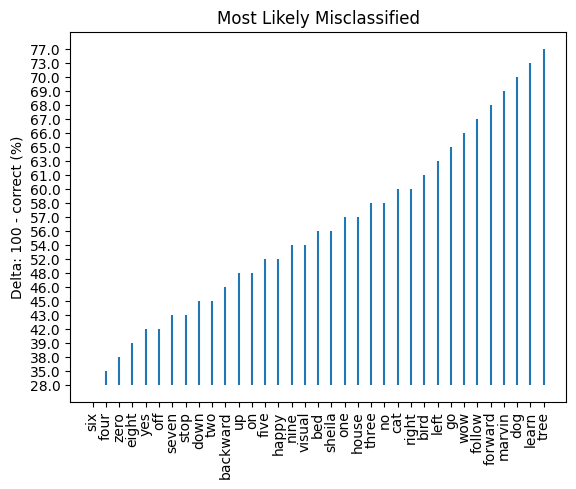
\includegraphics[width=0.48\textwidth]{mostmis.png}
        \caption{\small Most misclassified}
        \label{fig:mostmis}
    \end{figure}

    \begin{figure}[H]
        \centering
        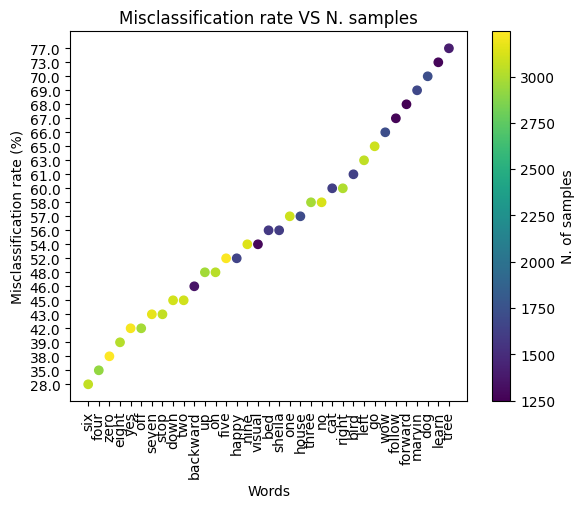
\includegraphics[width=0.48\textwidth]{correlation.png}
        \caption{\small Misclassified VS N. of samples}
        \label{fig:correlation}
    \end{figure}

\addcontentsline{toc}{subsection}{{Weights Visualization}}
\noindent
\textbf{Weights Visualization}\\
An interesting way to understand how the model works is to visualize the weights of the first layer, shown in figure \ref{fig:weights}. The red parts votes in favour of the specific
class, while the blue parts votes against it. The weights distribution is not uniform and changes from word to word, according to their spectrograms. Remembering that the spectrograms
has on y axis the frequency and on x axis the time, it is possible to notice on which frequencies the model focused. 
For example, the high frequencies strongly penalized words like \textit{Follow} and favours words like \textit{up} and \textit{wow}.
In the case of \textit{Forward}, \textit{Four} and \textit{Follow}, due to the similarity of their spectrograms, the model assigns almost the same weights to the same frequencies.
Indeed, the model learnt to extract relevant acoustic details, as shown by the overlapping between the assigned weights and the spectrograms of a specific
word (figure \ref{fig:spec_vs_weights}). 

    \begin{figure}[H]
        \centering
        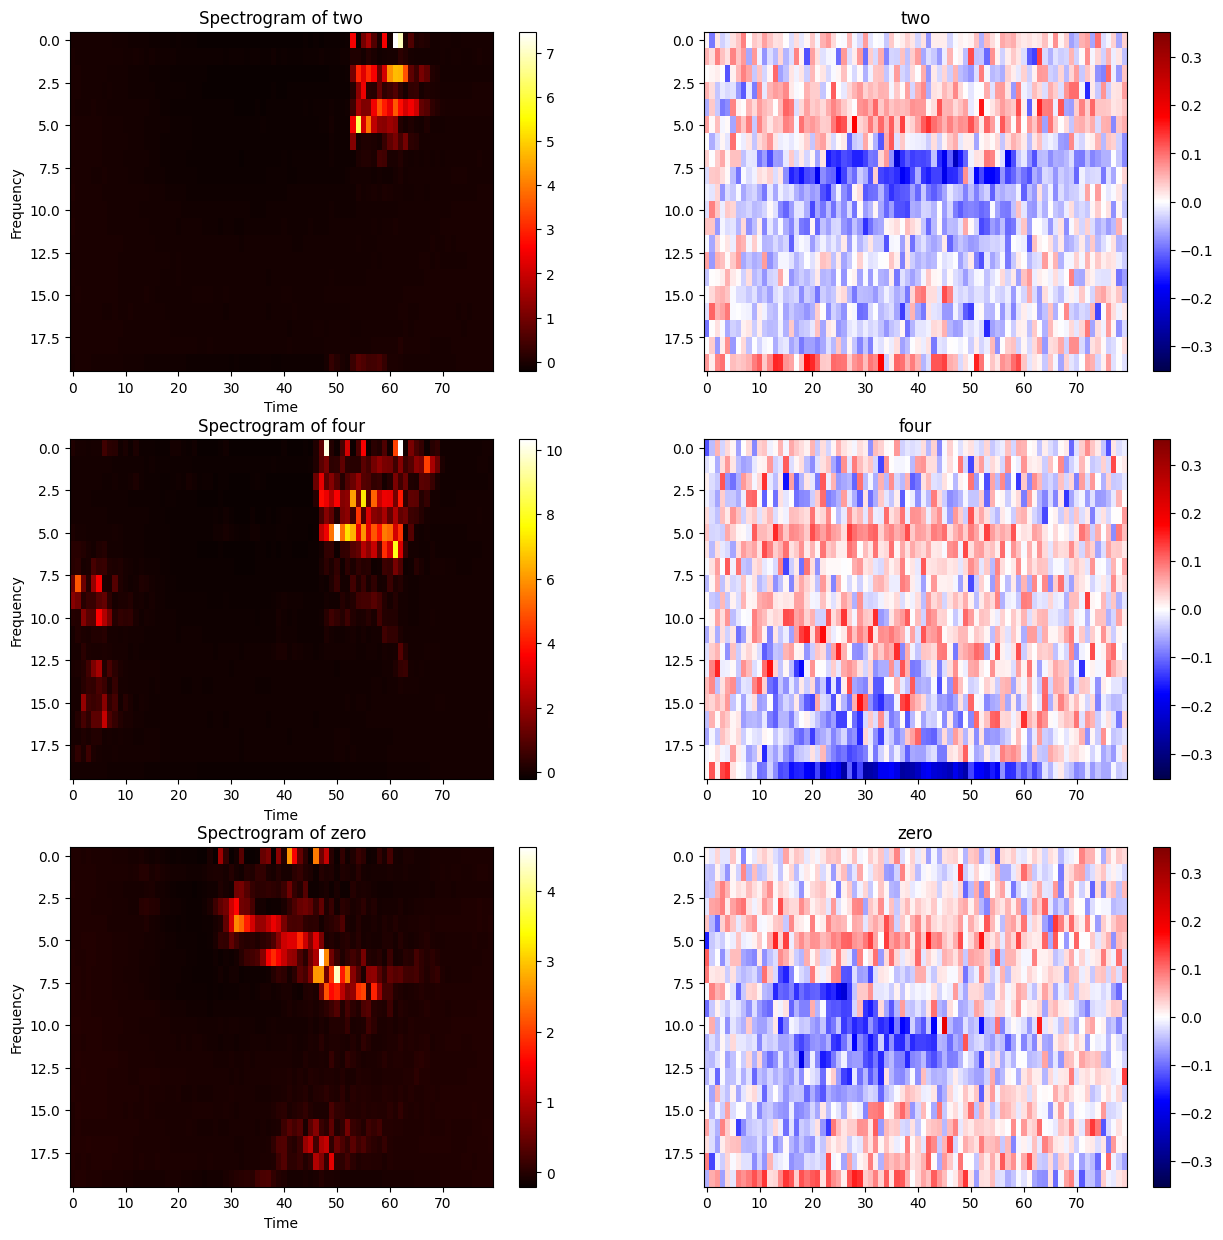
\includegraphics[width=0.48\textwidth]{spec_vs_weights.png}
        \caption{\small Spectrogram VS Weights}
        \label{fig:spec_vs_weights}
    \end{figure}

\end{multicols}

        \begin{figure}[H]
            \centering
            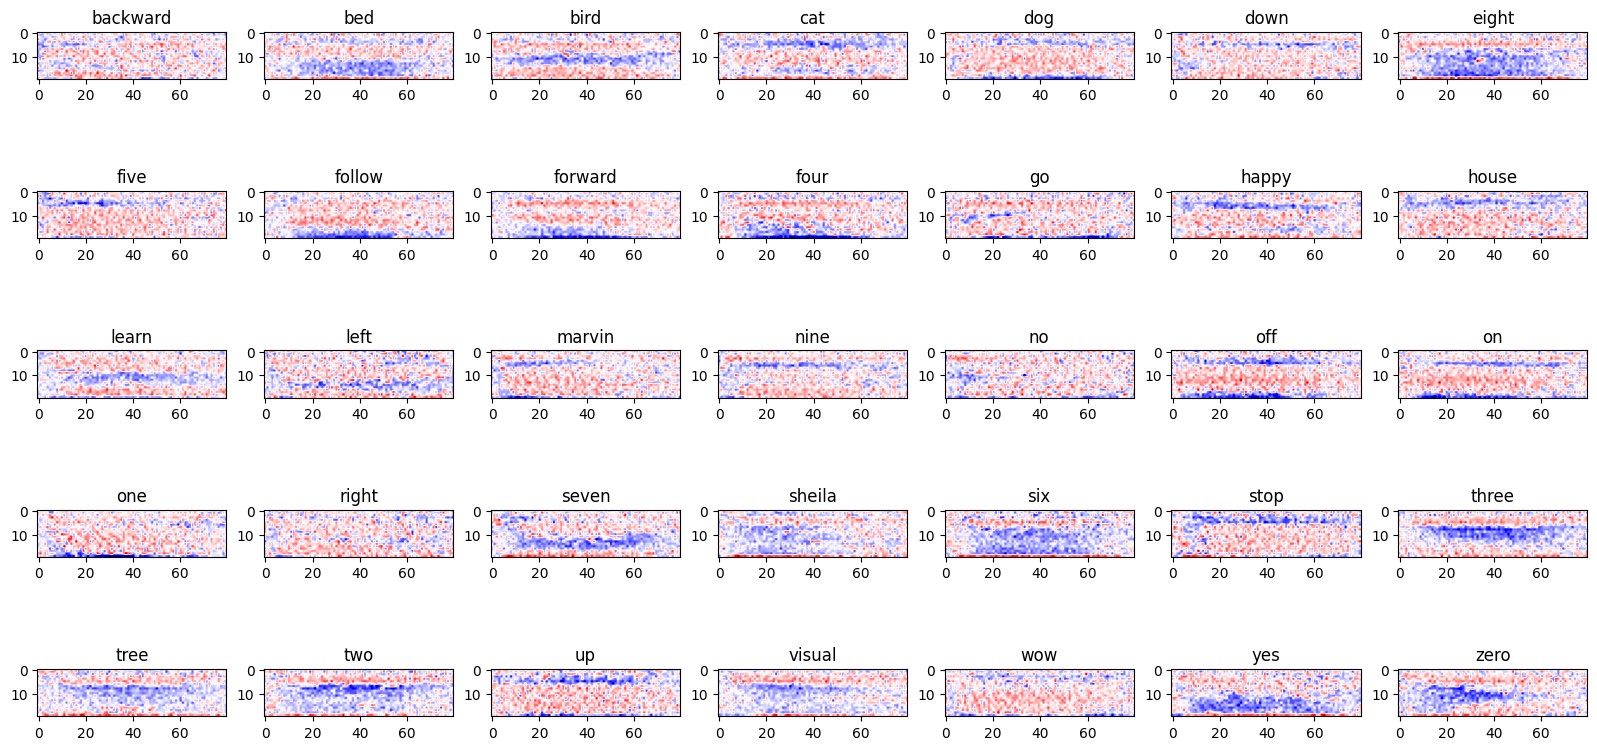
\includegraphics[width=0.83\textwidth]{weights.png}
            \caption{\small Weights visualization}
            \label{fig:weights}
        \end{figure}

        \begin{figure}[H]
            \centering
            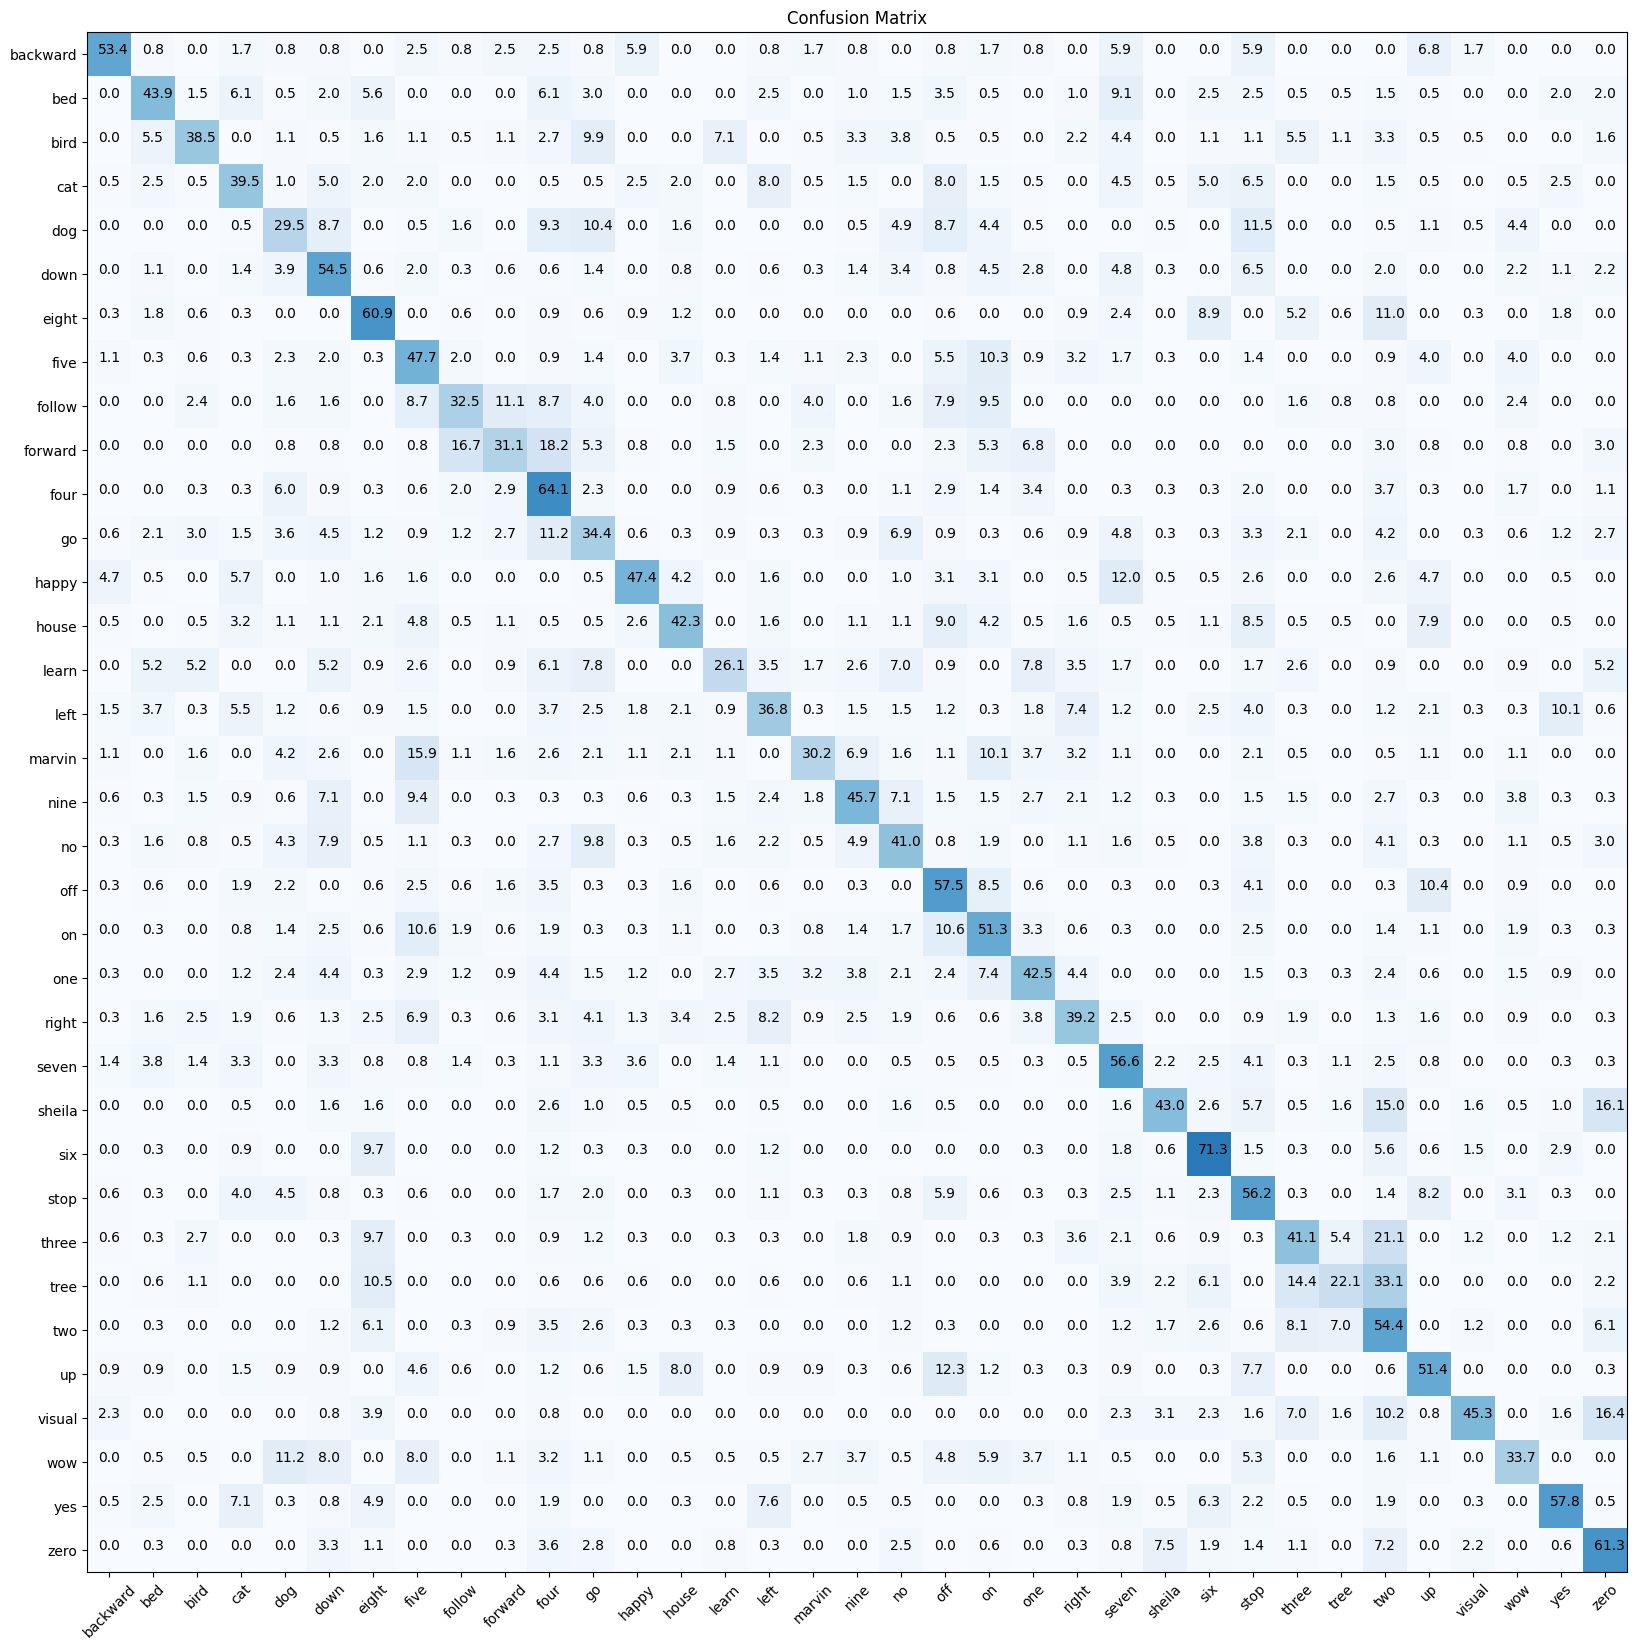
\includegraphics[width=0.83\textwidth]{confmat.png}
            \caption{\small Test accuracies comparison}
            \label{fig:confmat}
        \end{figure}


%-----------------------------------------------------------


\vfill
%\subsection*{\normalsize Declaration}
%I affirm that this report is the result of my own work and that I did not share any part of it with anyone else except the teacher.


\end{document}